\chapter{The Dataset: Collection, Preparation and Exploration}
\label{ch:data}

% un unico capitolo: raccolta -> preprocessing -> dataset finale -> analisi esplorativa in chiusura
This chapter follows the data from their three sources to the objects the models read:
what was collected and from where (\cref{sec:data:sources,sec:data:collection}), how
large and how reliable it is (\cref{sec:data:scale,sec:data:quality}), how the raw
streams were preprocessed (\cref{ch:prep}) and how the final dataset was defined
(\cref{sec:data:final}).  It closes with an exploratory and statistical analysis of the
data (\cref{ch:exploration}).

\section{The four tables}
\label{sec:data:sources}

The dataset covers twenty-one consecutive days, from 6 to 26 March 2026, and consists of
four tables (\cref{tab:data:sources}).  The \emph{markets} table describes every market
that existed in the period: question text, tags, the two outcome tokens, creation and
end dates, and the final outcome.  The \emph{order book} table is the stream of
price-level updates of the ``Yes'' side of every market's book: each row carries the
best bid and ask, the changed price level, size and side, and the mid price.  The
\emph{snapshots} table holds full order-book states.  The \emph{transactions} table is
the on-chain record of every fill: block number, timestamp, transaction hash, wallet,
role (maker or taker), token, side, quantity, price and fee.

\begin{table}[t]
\centering
\caption{Data sources.  Row counts from the DuckDB database.}
\label{tab:data:sources}
\begin{tabular}{lrl}
\toprule
Table & Rows & Content \\
\midrule
markets      & 175{,}476            & one row per market: text, tags, tokens, dates, outcome \\
order book   & 5{,}555{,}777{,}555  & price-level updates of the Yes-side book \\
snapshots    & 51{,}674{,}425       & full order-book states (JSON) \\
transactions & 218{,}882{,}492      & on-chain fills with wallet, token, side, size, price \\
\bottomrule
\end{tabular}
\end{table}

\section{Collection}
\label{sec:data:collection}

\subsection{Market metadata: the Gamma API}

The \emph{markets} table was built from Polymarket's public metadata service (the Gamma
API): the markets closed in the window were paged through its keyset endpoint, and the
markets that appear in the transactions but not in that listing were completed one by
one through the markets-by-token endpoint.  The tags are the source of the eight
categories used throughout the thesis (crypto, sports, esports, politics, weather,
economy and tech, culture, other).

\subsection{The order-book archive}

The \emph{order book} and \emph{snapshots} tables come from a public archive of the
operator's websocket feed published on Kaggle \cite{gozo2026polymarket}: one file per
day, restricted to the Yes side of every book, with the creation time and the reception
time of every message.

\subsection{The on-chain transactions: a blockchain scraper}

The \emph{transactions} table was collected with a modified version of
\path{poly-trade-scan} \cite{martkir2026polytradescan}, an open-source client that reads
every Polygon block from a public node, filters the transactions addressed to
Polymarket's exchange contracts and decodes their \texttt{matchOrders} calls; the
modified version emits one row per wallet and per fill.  \todo{details of the decoding
(taker and maker legs, fees), the node, the retries; 219 million rows are fill legs}

\section{Scale, coverage and storage}
\label{sec:data:scale}

Daily activity is stable over the period: 9.2--11.8 million transaction rows,
122{,}000--161{,}000 distinct wallets and 15{,}000--21{,}000 active markets per day.
The data are stored as Parquet files and queried with DuckDB \cite{raasveldt2019duckdb}.
\todo{storage sizes; a figure of the daily volumes}

\section{Data quality}
\label{sec:data:quality}

\todo{the facts about the data that shape every later choice, with the numbers:}
\begin{itemize}[nosep]
  \item fabricated mid on one-sided books (the feature builder substitutes $0.49$ or
  $0.51$ for the missing side);
  \item token orientation: the book refers to token~1 in Yes/No markets and to token~2
  in all the others, while the raw trade direction refers to token~1 everywhere;
  \item about 40\% of the samples have a mid below $0.05$ or above $0.95$;
  \item one dip in the transaction stream, on 20 March.
\end{itemize}

\section{Preprocessing and audit of the pipeline}
\label{ch:prep}

\subsection{Time axis: blocks and the synchronisation of the two streams}
\label{sec:data:blocks}

Polygon produces a block roughly every two seconds, and every transaction carries its
block number.  The block is the time step of the models: a step is one block, the set
of transactions in it, and the order-book updates that arrived since the previous
block.  Because the two streams are collected by different clocks, a model that acts at
block $t$ sees every book update created strictly before $t$ and the fills of the block
itself.

\subsection{Derived tensors}
\label{sec:data:tensors}

\todo{to write:}
\begin{itemize}[nosep]
  \item a 52-dimensional feature vector per market and per order-book update (best
  quotes, five levels per side, spread, mid, imbalances, recent trade statistics),
  stored in hourly partitions;
  \item the market lifecycle table: deployment time (known in advance) and last trade
  (hindsight only, used to define the samples and never as an input);
  \item static market features: a sentence embedding of the question and a few
  numeric fields;
  \item dense indices for markets and wallets.
\end{itemize}

\subsection{Audit of the pipeline}
\label{sec:data:audit}

\todo{the three errors found by the audit and fixed before any result (wrong price
column; leaky momentum baseline; incomplete label lookup), and what was retrained}

\section{The final dataset: labels, samples, features and periods}
\label{sec:data:final}

\subsection{Labels}
\label{sec:data:labels}

The target of a market $m$ at block time $t$ and horizon $H$ is the sign of the change
of its mid price:
\begin{equation}
  y_{m,t} = \operatorname{sign}\bigl(\operatorname{mid}_m(t+H) - \operatorname{mid}_m(t)\bigr) \in \{\textsc{down}, \textsc{const}, \textsc{up}\},
  \label{eq:label}
\end{equation}
where $\operatorname{mid}_m(s)$ is the mid price of the last order-book update of $m$
strictly before $s$.  Three classes, because over one hour the mid of more than half of
the samples does not move at all; no dead zone, any move of at least one tick counts;
when $t + H$ is beyond the loaded data the label is missing.  \todo{samples: one per
(market, block) with an update; the deduplicated view, one sample per market per
fifteen minutes}

\subsection{Feature engineering}
\label{sec:prep:features}

\todo{to write.  The feature tables:}
\begin{itemize}[nosep]
  \item the sixty-one hand-made causal features, in five groups: price history, book
  shape, activity and clock, on-chain trades, static fields of the market (the full
  list in \cref{app:features});
  \item sibling features: the contracts of the same event;
  \item news features: GDELT counts and tone for the entities named in the question;
  \item wallet features on the transaction edges;
  \item forecast features: the quantiles of a zero-shot Chronos-2 forecast.
\end{itemize}

\subsection{Training, validation and test periods}
\label{sec:data:splits}

The twenty-one days are split by date: models are trained on 6--12 March and every
design choice is taken on the validation day, 13 March; the period 24--26 March is a
locked test set, never evaluated and never inspected, reserved for the final numbers.

\section{Exploratory and statistical analysis}
\label{ch:exploration}

\todo{in closing, as agreed: what the data say before any model is trained, in three
parts.  Numbers on the training and validation days only.}

\subsection{The price process}
\label{sec:expl:price}

\todo{outline: the event stream and how uneven it is; how often a price moves at each
horizon (\cref{tab:expl:classes}); the price level; the activity clock; the direction
of a move; the kind of contract; the contracts of the same event; the wallets}

\begin{table}[t]
\centering
\caption{Share of the three classes among the labelled validation samples, by horizon.}
\label{tab:expl:classes}
\begin{tabular}{lccc}
\toprule
Horizon & \textsc{down} & \textsc{const} & \textsc{up} \\
\midrule
1 min  & 0.057 & 0.891 & 0.052 \\
15 min & 0.164 & 0.690 & 0.146 \\
1 h    & 0.236 & 0.549 & 0.215 \\
6 h    & 0.335 & 0.354 & 0.312 \\
12 h   & 0.377 & 0.275 & 0.348 \\
\bottomrule
\end{tabular}
\end{table}

\subsection{The transactions as a graph}
\label{sec:expl:graph}

\todo{size, density and degree distributions; components and $k$-cores; the graph in
time; a map of the graph (\cref{fig:graph:map:cat}); synchronous publics; what it says
for the models}

\begin{figure}[p]
\centering
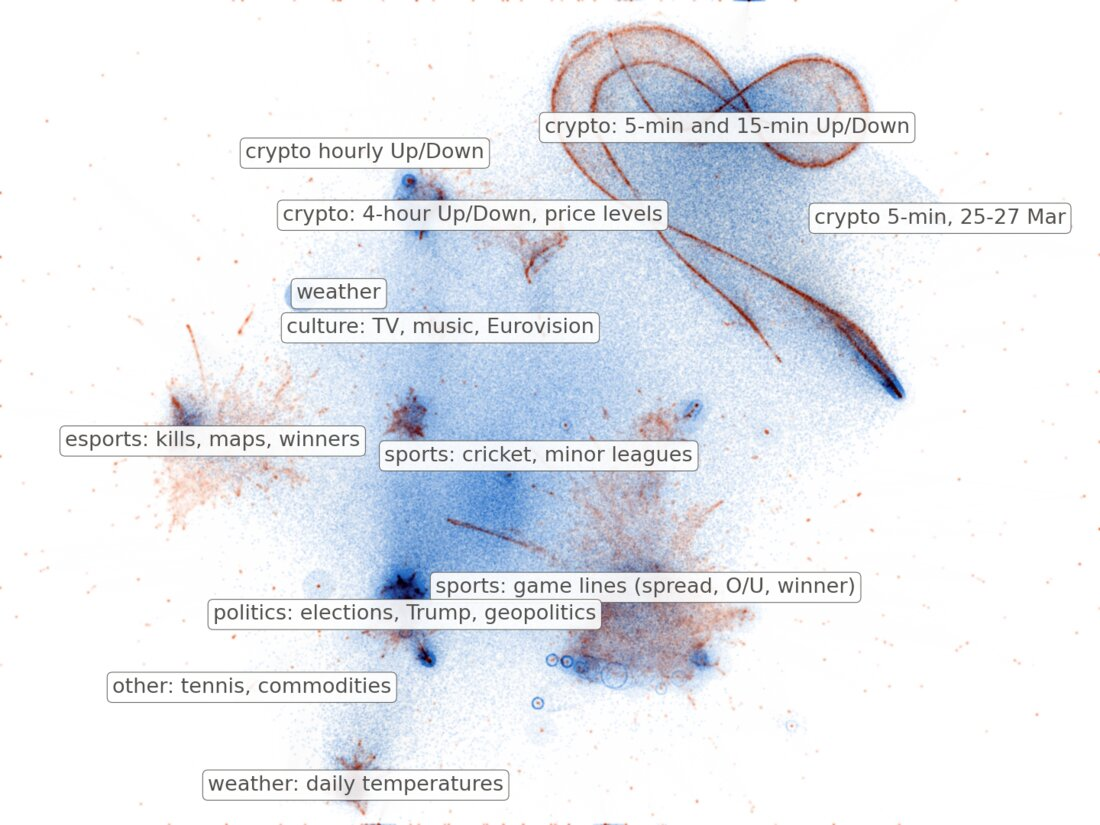
\includegraphics[width=\textwidth]{figures/graph/graph_map_category.jpg}
\caption{Three weeks of transactions as a graph: wallets (blue) and markets (orange),
joined by the trading relations between them, 6--26 March 2026.  \todo{caption}}
\label{fig:graph:map:cat}
\end{figure}

\subsection{The structure of the feature space}
\label{ch:structure}

\todo{data-mining study of the hand-made features: how many quantities they contain
(PCA, correlation blocks); maps of the samples (UMAP, t-SNE); linear, local and
threshold separability; families of markets; across the horizons}

\subsection{What the data say before a model is trained}
\label{sec:expl:agenda}

\todo{summary that sets the agenda of the methodology}
